\chapter{Integrál}
\section{Definice}
\subsection{Jednoduchá funkce}
Nechť $(X,\mathscr{U},\mu)$ je měřitelný prostor s mírou a $(Y,\mathscr{T})$ je topologický prostor reálných čísel $Y=\mathbb{R}$ s přirozenou topologií. Nechť dále platí, že $f:X\to Y$ je takové zobrazení, že $y=f(x)$ nabývá v $\mathbb{R}$ pouze konečně mnoha nezáporných a konečných hodnot $y_1,y_2, \ldots,y_n$

\begin{figure}
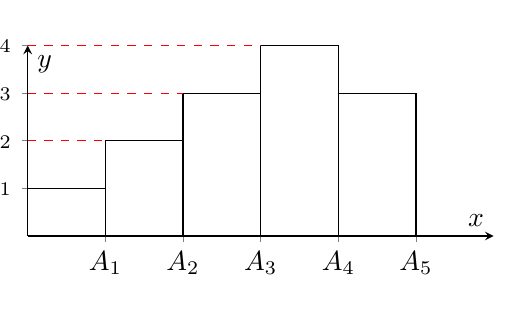
\begin{tikzpicture}[trim axis left, trim axis right]
		\begin{axis}[
		height=4cm,
		width = 7.5cm,
		%title=Bin�rn� relace,
		axis lines=middle,
		xlabel={$x$},
		ylabel={$y$},
		ymin=0, ymax=4,
		xmin=0, xmax=6,
		ytick = {0,1,2,3,4},
		xtick = {0,1,2,3,4,5},
		yticklabels = {0,$y_1$,$y_2$,$y_3$,$y_4$},
		xticklabels = {0,$A_1$,$A_2$,$A_3$,$A_4$,$A_5$}
		%grid = both
		]
		\addplot [no marks] table {
		0 1
		1 1
		1 0
		1 2
		2 2
		2 0
		2 3
		3 3
		3 0
		3 4
		4 4
		4 0
		4 3
		5 3
		5 0
		};
		\addplot [dashed, red] table {
		0 2
		1 2
		};
		\addplot [dashed, red] table {
		0 3
		2 3
		};
		\addplot [dashed, red] table {
		0 4
		3 4
		};
	\end{axis}
	\end{tikzpicture}
\caption{Průběh primitivní funkce (aproximace složitější funkce)}
\end{figure}

Pak funkce $f$ se nazývá \textbf{jednoduchou funkcí}. Označíme-li $A_i=\{x: f(x)=y_i\}, i=1,2,\ldots,n$, pak zřejmě patří, že $f(x)=\sum_{i=1}^n y_i\chi_i(x)$, kde $\chi_A$ je charakteristická funkce množiny $A$. Zobrazení $f$ je měřitelné, právě když $A_i, i=1,2,\ldots,n$ jsou měřitelné množiny.

\subsection{Integrál}
Nechť nyní $f:X\to Y$ je jednoduchá měřitelná funkce a nechť $E\in\mathscr{U}$. Pak integrál funkce $f$ na množině $E$ definujeme vztahem

\[ \int_E f\d \mu = \sum_{i=1}^{n}y_i \mu(A_i\cap E) \]

\textbf{Věta:} Nechť $f$ a $g$ jsou jednoduché měřitelné funkce. A nechť $C$ je nezáporná konstanta. Potom při daném zobrazení $f$ je zobrazení $S$,$S:\mathscr{U}\to\mathbb{R}$
\[ S(E) = \int_e f\d \mu \]

je mírou na množině $\mathscr{U}$ a platí
\[ \int_E C f\d \mu = C\int_E f\d \mu \]

a zároveň

\[ \int_E (f+g)\d \mu = \int_E f\d \mu + \int_E g\d \mu \]

\begin{note}{Důkaz}
Abychom dokázali, že $S$ je míra, stačí dokázat, že $S$ má patřičné vlastnosti. Je-li $A,B\subset \mathscr{U}, A\subset B$, pak $\mu(A)\leq \mu(B)$. Nechť $E,F\subset\mathscr{U}, E\subset F$, pak

\[ S(E) = \sum_{i=1}^{n}y_i\mu(A_i\cap E)\leq \sum_{i=1}^{n}y_i\mu(A_i\cap F)=S(E), \]

pak $S$ má vlastnost míry. Nyní se věnujme druhé vlastnosti míry, a tedy $A,B\in\mathscr{U}, A\cap B=\emptyset$, pak $\mu(A\cup B)=\mu(A) + \mu(B)$. Nechť tedy $E,F\in\mathscr{U}, E\cap F=\emptyset$, pak 
\begin{eqnarray*}
S(E\cup F) &=& \sum_{i=1}^{n}y_i\mu\big(A_i\cap (E\cup F)\big) = \sum_{i=1}^{n}y_i\mu\big((A_i\cap E)\cup (E\cap F)\big)=\\
&=& \sum_{i=1}^{n}y_i \mu(A_i\cap E)+\mu(A_i\cap F)=\sum_{i=1}^n y_i\mu(A_i\cap E) + \sum_{i=1}^n y_i\mu(A_i\cap F)=\\
&=& S(E) + S(F), \text{$S$ je mírou $\mathscr{U}$}
...\end{eqnarray*}

Nyní se věnujme druhému tvrzení
\[ \int_E C f\d \mu = \sum_{i=1}^{n} C y_i\mu (A_i\cap E)=C\sum_{i=1}^n y_i\mu(A_i\cap E)=C\int_E f\d \mu \]

Nyní se věnujme tvrzení, že 
\[ \int (f+g) = \int f + \int g \]

Předpokládejme, že jednoduchá funkce $g$ nabývá hodnot $z_1,z_2,\ldots, z_m$. Příslušné množiny, na níž nabývá těchto hodnot pak označíme symbolem $B_j, B_j=\{x: g(x)=z_j\},j=1,2,\ldots,m $.\br

Funkce $f$ nabývá konstantních hodnot $y_i$ na množině $A_i$ a funkce $g$ konstantní hodnoty $z_j$ na množině $B_j$. A $f+g$ nabývá konstantní hodnoty $y_i+z_j$ na množině $E_{i,j}=A_i\cap B_j$.
\[ \int_E (f+g)\d \mu = (y_i+z_j)\mu(E_{i,j})=y_i\mu(E_{i,j}+z_j\mu(E_{i,j}) \]

Přičemž
\[ \int_{E_{i,j}} f\d \mu + \int_{E_{i,j}} g\d \mu, \]
kde $E_{i,j}$ jsou disjunktní a platí $X=\bigcup_{i=1}^n\bigcup_{j=1}^m E_{i,j}$, pak vzhledem k tvrzení, že $S$ je míra.

\begin{eqnarray*}
\int_X (F+g)\d \mu &=& \sum_{i=1}^n\sum_{j=1}^m\int_{E_{i,j}}(f+g)\d \mu =\\
&=&\sum_{i=1}^n\sum_{j=1}^m \left( \int_{E_{i,j}}f\d \mu + \int_{E_{i,j}}g\d \mu\right)=\\
&=& \sum_{i=1}^n\sum_{j=1}^m\int_{E_{i,j}}f\d \mu + \sum_{i=1}^n\sum_{j=1}^m\int_{E_{i,j}}g\d \mu
\end{eqnarray*}

Pak platí
\[ \int_X f\d \mu + \int_X g\d \mu \]

Všechna tvrzení věty jsme dokázali!
\end{note}

Našli jsme některé elementární vlastnosti integrálu jednoduchých funkcí. V praxi asi budou složitější.

\begin{figure}
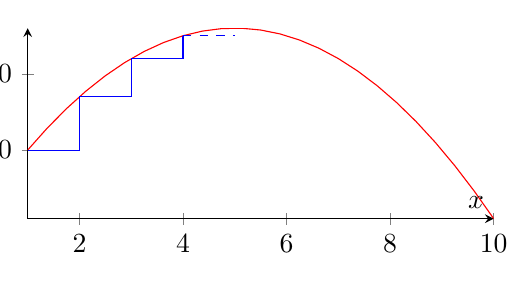
\begin{tikzpicture}[trim axis left, trim axis right]
		\begin{axis}[
		height=4cm,
		width = 7.5cm,
		axis lines=middle,
		xlabel={$x$},
		ylabel={$y$},
		ylabel near ticks
		%grid = both
		]
		\addplot [red, domain=1:10] {
			-x^2 + 10*x+ 1
		};
		\addplot [blue, no marks] table {
			1 10
			2 10
			2 17
			3 17
			3 22
			4 22
			4 25
		};
		\addplot [blue, dashed] table {
			4 25
			5 25
		};
	\end{axis}
	\end{tikzpicture}
\caption{Aproximace složitějších funkcí pomocí jednoduchých funkcí}
\end{figure}

Jednoduchými funkcemi se můžeme libovolně přiblížit ke každé složitější funkci. Platí debaseyova věta.

\subsection{Debaseyova věta}
Nechť $f_1,f_2,\ldots,f_n$ je nekonečná posloupnost jednoduchých měřitelných funkcí na měřitelném prostoru $(X,\mathscr{U})$ takových, že pro každé $x\in X$ platí:
\[ 0\leq f_1(x) \leq f_2(x)\leq \ldots \leq f(x)<\infty\]
\[ \lim_{n\to\infty} f_n(x) = f(x), \]

pak funkce $f$ je měřitelná a platí 
\[ \lim_{n\to\infty} \int_X f_n\d \mu = \int_X f\d \mu
\]

Tímto se rozšiřuje množina integrovatelných funkcí.

\subsection{Rozšíření}
Další rozšíření dostaneme, jestliže budeme definici integrace mít i pro funkce, které mohou nabývat i záporných hodnot. Lze postupovat tak, že k dané funkci $f$ zavedeme funkci $f^+$ a to bude maximum $f$, tedy $f^+=\max(f,0)$, resp. $f^-=-\min(f,0)$.

\begin{figure}
\begin{tikzpicture}[trim axis left, trim axis right]
		\begin{axis}[
		height=6cm,
		width = 7.5cm,
		axis lines=middle,
		xlabel={$x$},
		ylabel={$y$},
		legend style={at={(axis cs:190,1)},anchor=north west},
		ylabel near ticks
		%grid = both
		]
		\addplot [red, domain=1:180] {
			-cos(x)
		};
		\addplot [blue, dashed, domain=1:180] {
			abs(-cos(x))
		};
		\addplot [magenta, dotted, domain=0:90] {
			0
		};
		\addplot [magenta, dotted, domain=90:180] {
			-cos(x)
		};
		\legend{$f$, $f^+$, $f^-$}
	\end{axis}
	\end{tikzpicture}
\caption{Popis obrázku}
\end{figure}


Funkce $f^+$ a $f^-$ jsou samozřejmě nezáporné a je-li $f$ měřitelné, jsou měřitelné i funkce $f^+$ a $f^-$. Přitom platí $f=f^+-f^-$. Dále bude užitečné se omezit na integrály konečné. Nechť tedy $(X,\mathscr{U},\mu)$ je měřitelný prostor s mírou a $(Y,\mathscr{T})$ topologický prostor reálných čísel s přirozenou topologií. Pak $f:X\to Y$ je funkce, která nabývá kladných i záporných hodnot. Je-li $f$ měřitelné, absolutní hodnota je $|f|=f^+ + f^-$.\br

Soubor všech takových funkcí $f$, pro které platí
\[ \int_X |f|\d \mu<\infty \]

nazveme souborem \textbf{Lebesgueho integrovatelných funkcí} na prostoru s mírou $(X,\mathscr{U},\mu)$, který označíme symbolem $\mathscr{L}^1(\mu)$. Integrál funkce $f\in\mathscr{L}^1(\mu)$ definujeme nyní vztahem

\[ \int_E f\d \mu = \int_E f^+\d \mu - \int_E f^-\d \mu \]

pro každou měřitelnou množinu $E\in\mathscr{U}$.\br

Z definice integrálu je zřejmé, že pro libovolná reálná čísla $\alpha,\beta$ a pro libovolné funkce $f$ a $g$ patřící do $\mathscr{L}^1, f,g\in\mathscr{L}^1$ je $\alpha f + \beta g\in\mathscr{L}^1$, přičemž platí

\[ \int_X(\alpha f + \beta g)\d \mu = \alpha\int_X f\d \mu + \beta\int_X g\d \mu \]

\begin{note}{Poznámka}
Ze vztahu
\begin{equation}
S(E) = \int_E f\d \mu
\label{eq: int_SE}
\end{equation}

a Libesgueovy věty je zřejmé, že pro každou nezápornou integrovatelnou funkci $f: X\to\mathbb{R}$ je vztah (\ref{eq: int_SE}) mírou na měřitelném prostoru $(X,\mathscr{U})$. Speciálně pro $f(x)=1, x\in X$ platí
\[ \mu(E)=S(E)=\int_E\d \mu \]
\end{note}

Položme nyní speciálně $(X, \mathscr{U})=(\mathbb{R},\mathscr{B}))$ a zvolme $\d \mu=\d x$. Pak pro $E=\langle a, x\rangle$ lze psát

\[ S(x) = \int_a^x f\d x, \]

kde $S(xú$ je mírou na $(\mathbb{R},\mathscr{B})$, pro níž platí, že pro každou množinu $E\in\mathscr{B}$, pro kterou $\mu(E)=0$ je také $S(E)=0$.

\[ f=\frac{\d  f}{\d  x} \]

Důležitá je také skutečnost, že toto tvrzení lze obrátit. Je-li míra $S$ na $\mathscr{U}$ absolutně spojitá vzhledem k míře $\mu$, platí implikace

\[ \mu(E) = 0 \Rightarrow S(E) = 0 \]

pak na $(\mathbb{R},\mathscr{B})$ existuje taková měřitelná funkce $f$, že míru $S(E)$ lze vyjádřit jako

\[ S(E) = \int_a^x f\d x \]

\subsection{Radonova-Nikodinova věta}
Nechť jsou na měřitelném prostoru $(X,\mathscr{U})$ dány konečné množiny $\mu$ a $S$ a nechť míra $S$ je absolutně spojitá vzhledem k míře $\mu$ (platí implikace $\mu(E) = 0 \Rightarrow S(e) = 0$). Pak na měřitelném prostoru $(X,\mathscr{U})$ existuje integrál funkce $f$, pro kterou platí

\[ S(E) = \int_E f\d \mu \]

Funkce $f$ se nazývá \textbf{derivací} míry $S$ dle míry $\mu$ a značí se symbolem

\[ \frac{\d  S}{\d \mu} \]

Přitom je zřejmé, že tato funkce není určena jednoznačně. Je-li však $f'$ libovolná jiná funkce, která vyhovuje daným požadavkům, pak se od funkce $f$ liší nanejvýš na množině nulové míry. Takže funkce jsou si rovny skoro všude vzhledem k míře $\mu$.